\chapter{Fallbeispiel}
In diesem Kapitel werden die Erkenntnisse aus den beiden vorangehenden Kapiteln genutzt, um das Poisson Problem $\Delta u = 1, u|_{\p \Omega} = 0$ einmal auf einem L-förmigen Gebiet   
\[
\Omega_L = [-1,1]^2 \cap \left\{ r(\cos\phi,\sin\phi)| r\in\R,0<\phi<\frac{3 \pi}{2} \right\}
\]
und einmal auf einem kreuzförmigen Gebiet
\[
\Omega_\times = ([-0.5,0.5] \times [-1,1]) \cap ([-1,1]\times[-0.5,0.5])
\]
zu approximieren. Es wird also der adaptive Gitteralgorithmus auf eine Anfangstriangulierung $\mathscr{T}_0$ angewendet, um eine Folge von Triangulierungen und Approximationen auf diesen Triangulierungen zu erhalten. Als Verfeinerungsverfahren wird das Rot-Grün-Blau-Verfahren genutzt. Für $\Omega_L$ ist $\mathscr{T}_0$ mit zugehöriger Approximation in Abbildung \ref{grid} für $\Omega_\times$ in Abbildung \ref{grid2} zu sehen.
\begin{figure}[!htbp]
	\begin{center}
		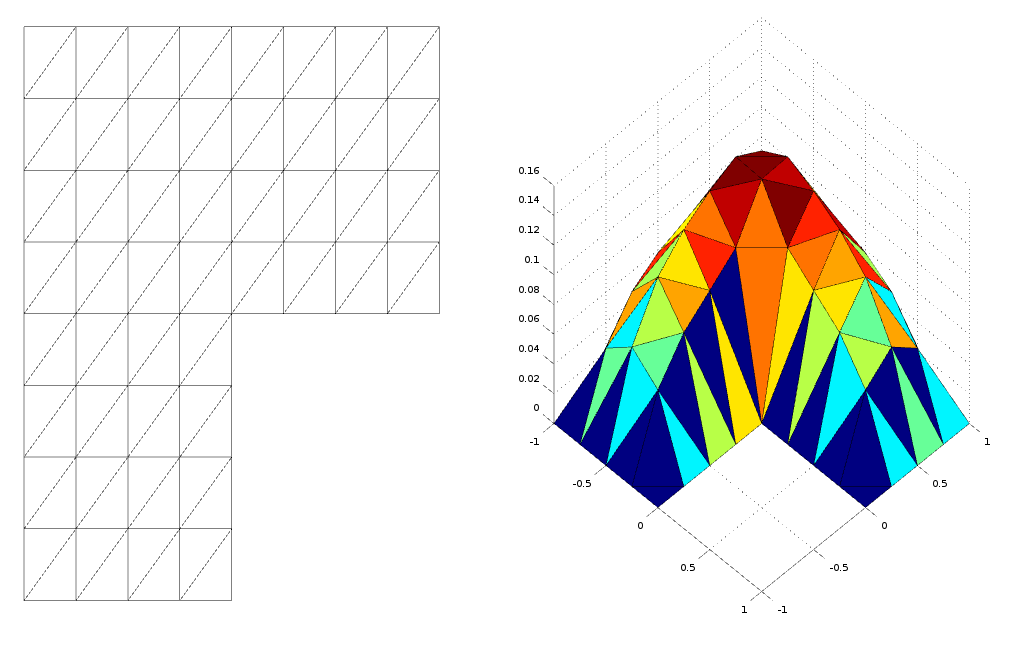
\includegraphics[width=11.2cm]{pics/nonref.png}
	\end{center}
	\caption{\label{grid}Triangulierung eines L-förmigen Gebiets (links). Approximierung einer Lösung des Poisson-Problems (rechts).}
\end{figure}
\begin{figure}[!htbp]
	\begin{center}
		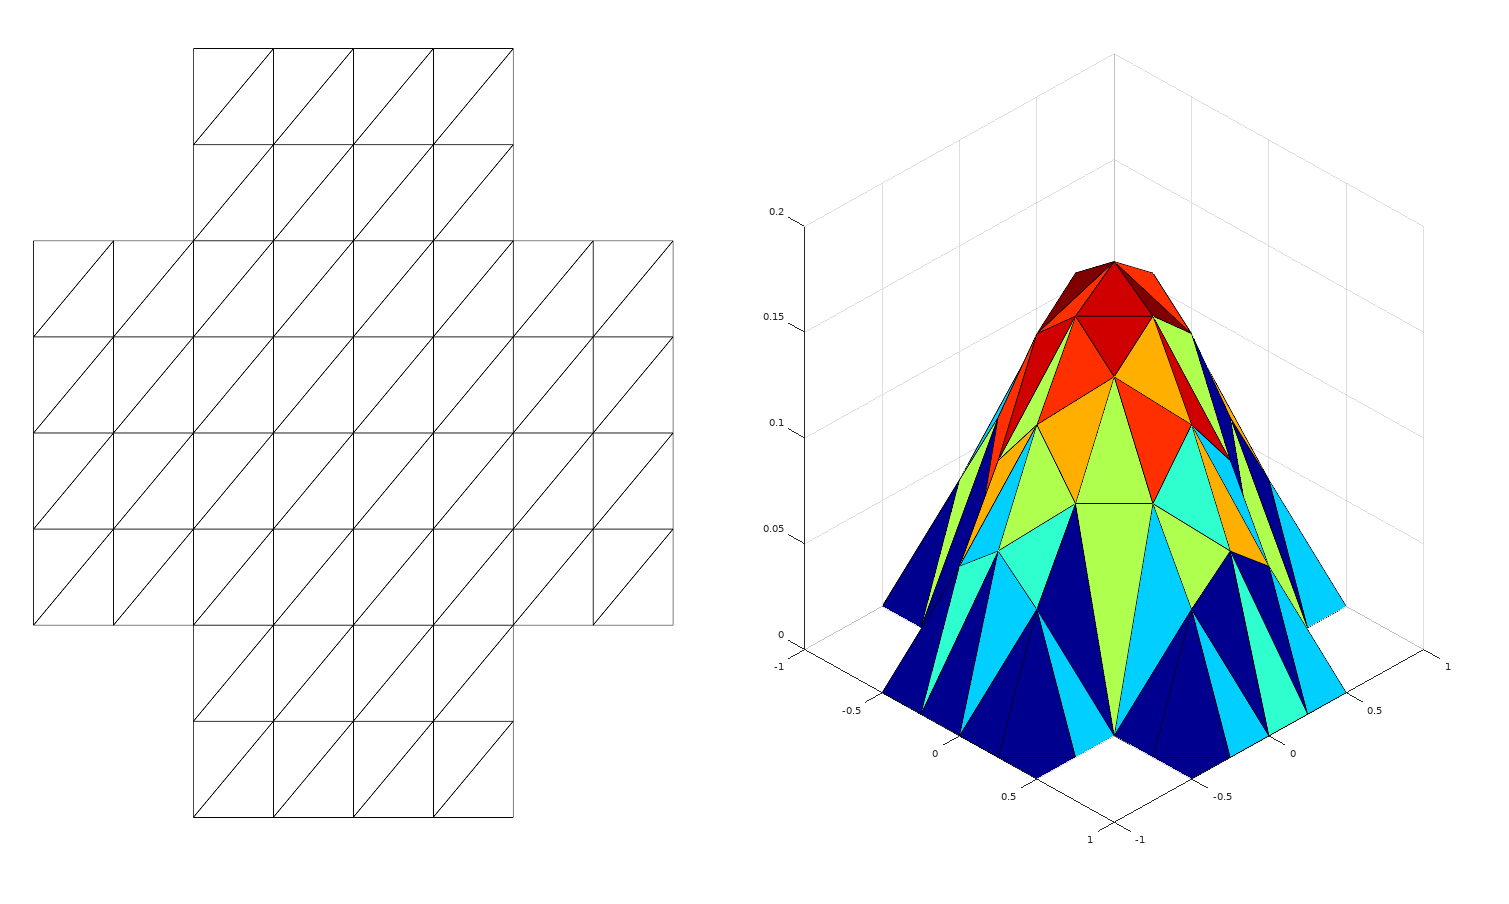
\includegraphics[width=13cm]{pics/nonref2.png}
	\end{center}
	\caption{\label{grid2}Triangulierung eines kreuzförmigen Gebiets (links). Approximierung einer Lösung des Poisson-Problems (rechts).}
\end{figure}
\section{Implementierung}
Im Folgenden ist eine Implementierung des adaptiven Gitteralgorithmus in \matlab \: zu finden. In Abbildung \ref{main} ist das Hauptprogramm zu sehen. Die Matrix c4n (coordinates for nodes) enthält in der i-ten Zeile die x und y Koordinate des i-ten Knotens im Gitter. Die Matrix n4e (nodes for elements) enthält in der i-ten Zeile die Nummern der Knoten, die zu dem i-ten Element gehören. Dabei ist die Kante vom ersten zum dritten Knoten die Längste. Diese Konvention wird für das Rot-Grün-Blau-Verfahren benötigt. Db (Dirichlet bondary) gibt in diesem Fall den Rand des Gebiets vor, da der Neumann-Rand leer ist. In jeder Zeile stehen die Nummern der Knoten, die zu einer Kante auf dem Rand gehören. \\
Das Unterprogramm $\texttt{comp\_estimators}$, zu sehen in Abbildung \ref{indi}, berechnet die Verfeinerungsindikatoren
\[
\eta^2_T(u_k) = h^2_T\|f\|^2_{L^2(T)} + \sum_{S\subset\p T} h_S\|\llbracket \nabla u_k \cdot n_S\rrbracket\|^2_{L^2(S)} 
\]
unter Benutzung der Abschätzung $h_T^{d-2}|S| \leq ch_S$.
Als Menge der zu verfeinernden Elemente wird vereinfachend
\[
M_k = \{T\in\mathscr{T}_k | \eta_T(u_k)\geq \Theta \max_{T'\in \mathscr{T}_k} \eta_{T'}(u_k)\}
\]
benutzt. $M_k$ ist damit in jedem Fall nicht leer, außer $u_k$ ist bereits die exakte Lösung. \\
Das Unterprogramm $\texttt{sides}$, in Abbildung \ref{indi} unten, liefert eine Datenstruktur für $\mathscr{S}_k$ die in $\texttt{comp\_estimators}$ verwendet wird. In n4s (nodes for sides) befindet sich in der i-ten Zeile die Knoten der i-ten Seite. Diese Nummerierung der Seiten wird benutzt, um in s4e (sides for elements) jedem Dreieck seine Seiten zuzuordnen und in e4s (elements for sides) jeder Seite die zwei anliegenden Elemente oder, wenn die Seite auf dem Rand liegt, das eine anliegende Element zuzuweisen.

\begin{figure}[!htbp]
	\lstinputlisting{codes/p1_adaptive.m}
	\caption{ \label{main}Hauptprogramm des adaptiven Gitteralgorithmus (oben). Konstruktion der Finite-Elemente Verfahrensmatrix (unten).}
\end{figure}
\begin{figure}[!htbp]
	\lstinputlisting{codes/p1_adaptive3.m}
	\caption{\label{indi}Berechnung der Verfeinerungsindikatoren}
\end{figure}

\begin{figure}[!htbp]
	\lstinputlisting{codes/p1_adaptive2.m}
	\caption{\label{redref} \matlab-Implementation der Rot-Grün-Blau-Verfeinerung}
\end{figure}
\newpage \newpage \newpage  
\section{Vergleich von Gitterfolgen}
\begin{table}[!htbp]
	\begin{tabular}{r|c|c|c}
		$\Theta\setminus\varepsilon_{stop}$& $2\cdot10^{-1}$ & $1\cdot10^{-1}$&$5\cdot10^{-2}$ \\
		\hline
		0,2&6,5s, 988Kn, 5 Schritte&30s, 4114Kn, 8 Schritte&2min15s, 16356Kn, 11 Schritte\\	
		0,4&9,6s 1478Kn, 7 Schritte&25,2s, 3730Kn, 9 Schritte&2min43s, 21394Kn,  13 Schritte\\
		0,5&7,6s, 1105Kn, 7 Schritte&31,4s, 4269Kn, 10 Schritte&2min8s, 16668Kn, 13 Schritte\\
		0,6&6,3s, 971Kn, 7 Schritte&28,7s, 3954Kn, 10 Schritte&1min46s, 15359Kn,  13 Schritte\\
		0,8&11,8s, 968Kn, 13 Schritte&51,6s, 3422Kn, 19 Schritte&3min19s, 12770Kn,  26 Schritte\\
		\hline
		Vergleich&6,8s, 3201Kn&29s, 12545Kn&1min48s, 49665Kn\\
	\end{tabular}
	\caption{\label{Test}Werte aus Messreihe für das L-förmige Gebiet mit verschiedenen Parametern für $\Theta$ und die Abbruchbedingung $\varepsilon_{stop}$. Es wird die benötigte Zeit für das Verfahren, sowie die Anzahl der Knotenpunkte (Kn) in der letzten Triangulierung und Iterationsschritte angezeigt. Als Vergleich ist die Approximation auf einem Gitter mit gleichmäßiger Gitterweite angegeben. Die Zeit entspricht daher der Zeit einer Approximation.}
\end{table}
\begin{table}[!htbp]
	\begin{tabular}{r|c|c|c}
		$\Theta\setminus\varepsilon_{stop}$& $2,2\cdot10^{-1}$ & $1,3\cdot10^{-1}$&$8\cdot10^{-2}$ \\
		\hline
		0,2&17,1s, 2377Kn, 6 Schritte&40,6s, 5927Kn, 8 Schritte&1min42s, 13385Kn, 10 Schritte\\	
		0,4&9,1s 1303Kn, 6 Schritte&33,4s, 4659Kn, 9 Schritte&1min23s, 10769Kn,  11 Schritte\\
		0,5&11s, 1575Kn, 7 Schritte&47,8s, 6455Kn, 10 Schritte&1min58s, 13749Kn, 12 Schritte\\
		0,6&10,4s, 1393Kn, 7 Schritte&38,7s, 5323Kn, 10 Schritte&1min31s, 11949Kn,  12 Schritte\\
		0,8&17s, 1671Kn, 11 Schritte&48,1s, 4017Kn, 15 Schritte&2min31s, 10945Kn,  20 Schritte\\
		\hline
		Vergleich&9,3s, 3201Kn&37,6s, 12545Kn&2min28s, 49665Kn\\
	\end{tabular}
	\caption{\label{Test2}Werte aus Messreihe für das kreuzförmige Gebiet $\Omega_\times$}
\end{table}
Wird das vorgestellte \matlab \:Programm auf die Anfangstriangulierungen für $\Omega_L$ (Abbildung \ref{grid}) und $\Omega_\times$ (Abbildung \ref{grid2}) angewendet, so entstehen Gitterfolge. Werden verschieden Werte für $\Theta$ verwendet, so werden verschiedene Elemente markiert und es entstehen unterschiedliche Gitterfolgen. In der Tabelle \ref{tabelle} sind die Triangulierungsfolgen für $\Theta =0,2/0,4/0,5/0,6 \text{ und } 0,8$ zu sehen. \\
Es ist zu beobachten, dass für $\Theta = 0,2$ fast alle Elemente im ersten Schritt markiert wurden. Im Gegensatz dazu wurde für $\Theta = 0,8$ nur ein einziges Element im ersten Schritt markiert. Bei allen Folgen ist eine starke Dichte an Elementen in den Ecken, besonders der einspringenden Ecke, zu erkennen. Für eine Abwägung welcher Wert für Theta am effizientesten ist, spielt jedoch vor allem die Rechenzeit und der Fehler der Approximation eine Rolle. In den Tabellen \ref{Test} und \ref{Test2} sieht man Daten einer Messreihe für beide Gebiete. In beiden Messungen fällt auf, dass mit steigendem Theta die Anzahl der Knoten in der letzten Triangulierung sinkt. Da in jedem Iterationsschritt ein Gleichungssystem mit \#Knoten vielen Gleichungen gelöst wird, liegt das Approximieren auf einem Gitter in $\mathcal{O}(\#Knoten^2)$. Somit sinkt die Zeit zur Berechnung der letzten Approximation mit steigendem Theta. Allerdings ist auch zu sehen, dass mit Theta die Anzahl der Iterationsschritte, die benötigt werden, um eine Fehlerschwelle zu unterschreiten, steigt.\\
Beim Vergleich mit einer Approximation auf einem Gitter mit gleichmäßiger Gitterweite fällt auf, dass hierfür sehr viel mehr Knoten gebraucht werden, um dieselbe Fehlerschwelle zu unterschreiten. Die Rechenzeiten sind jedoch im Fall von $\Omega_L$ vergleichbar, wenn nicht sogar geringer, da nur eine und nicht wie im Fall vom adaptiven Gitteralgorithmus eine ganze Reihe von Approximationen durchgeführt werden muss. Im Gegensatz dazu können sich im Fall von $\Omega_\times$ die adaptiven Gitter vor allem für kleine Fehler durchsetzen.\\



\begin{table}[!htbp]
	\begin{tabular}{c}
		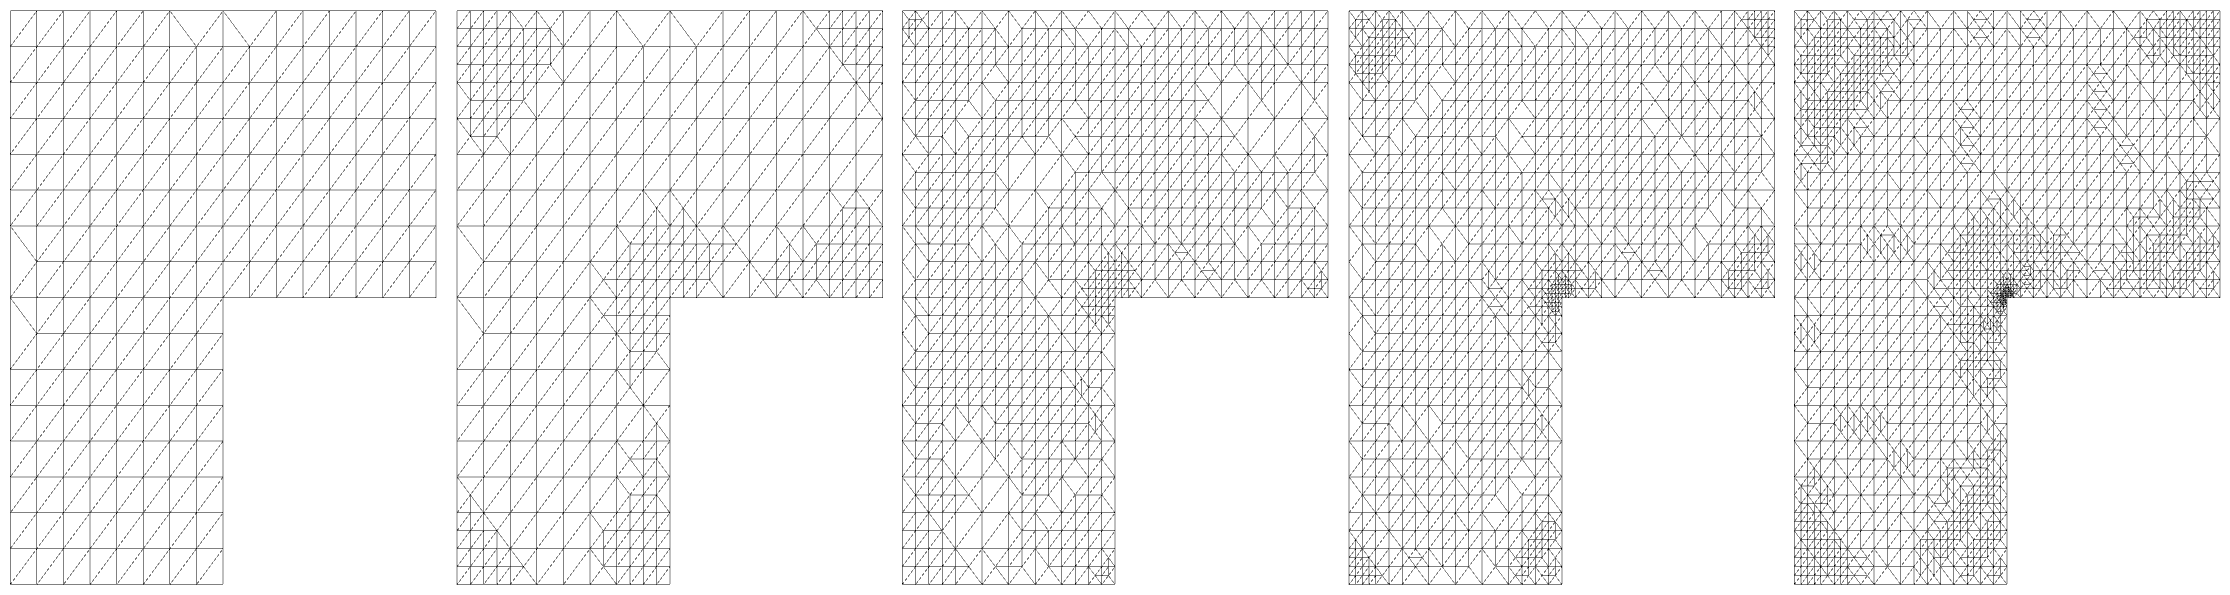
\includegraphics[width=16.5cm,height=3.5cm]{pics/grid02.png} \\
		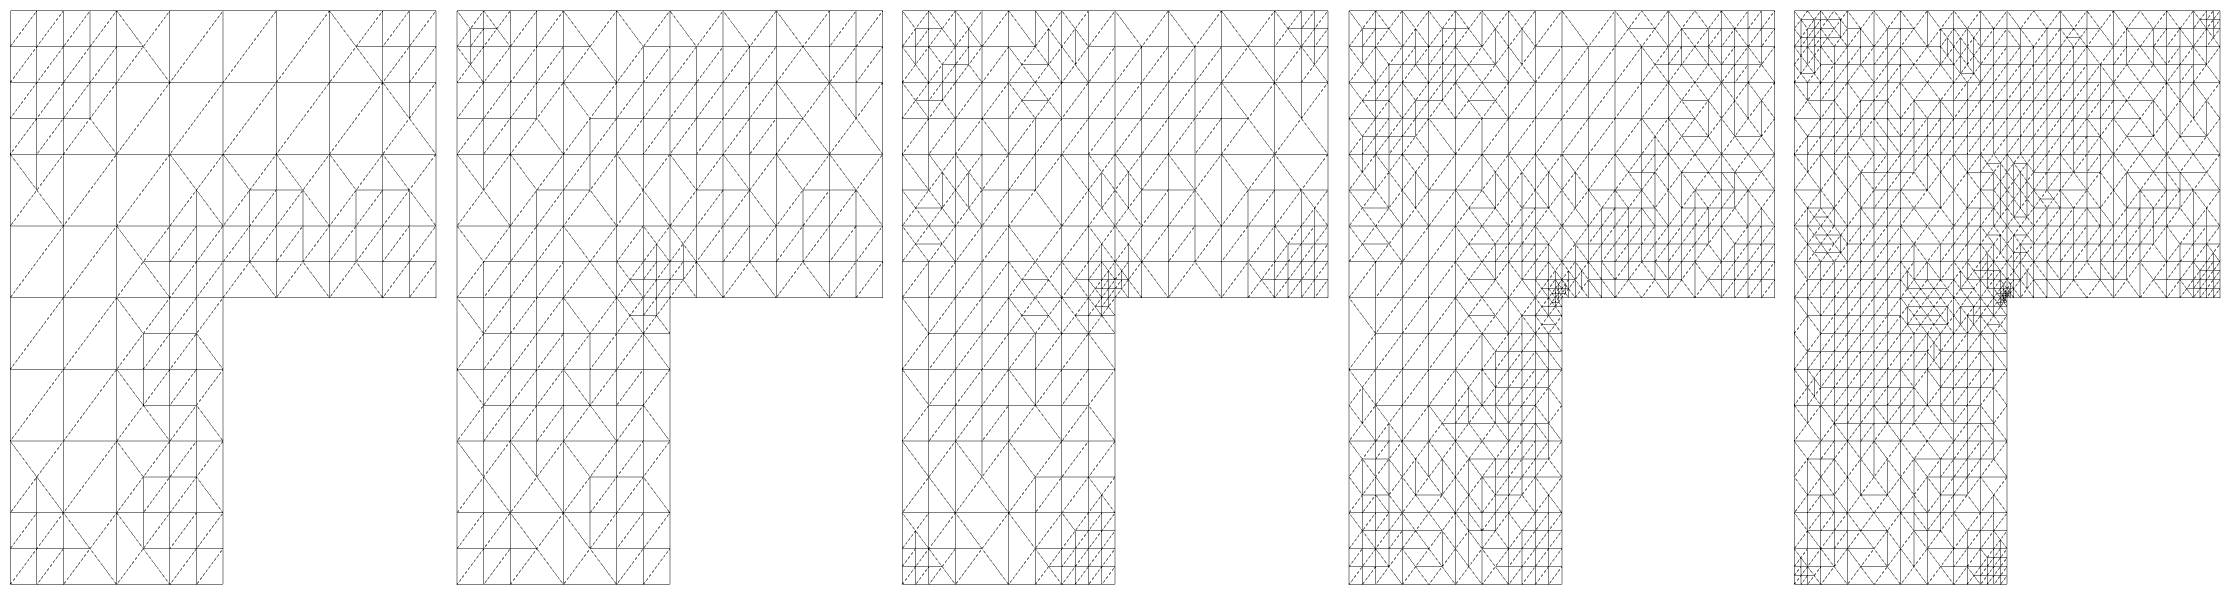
\includegraphics[width=16.5cm,height=3.5cm]{pics/grid04.png} \\
		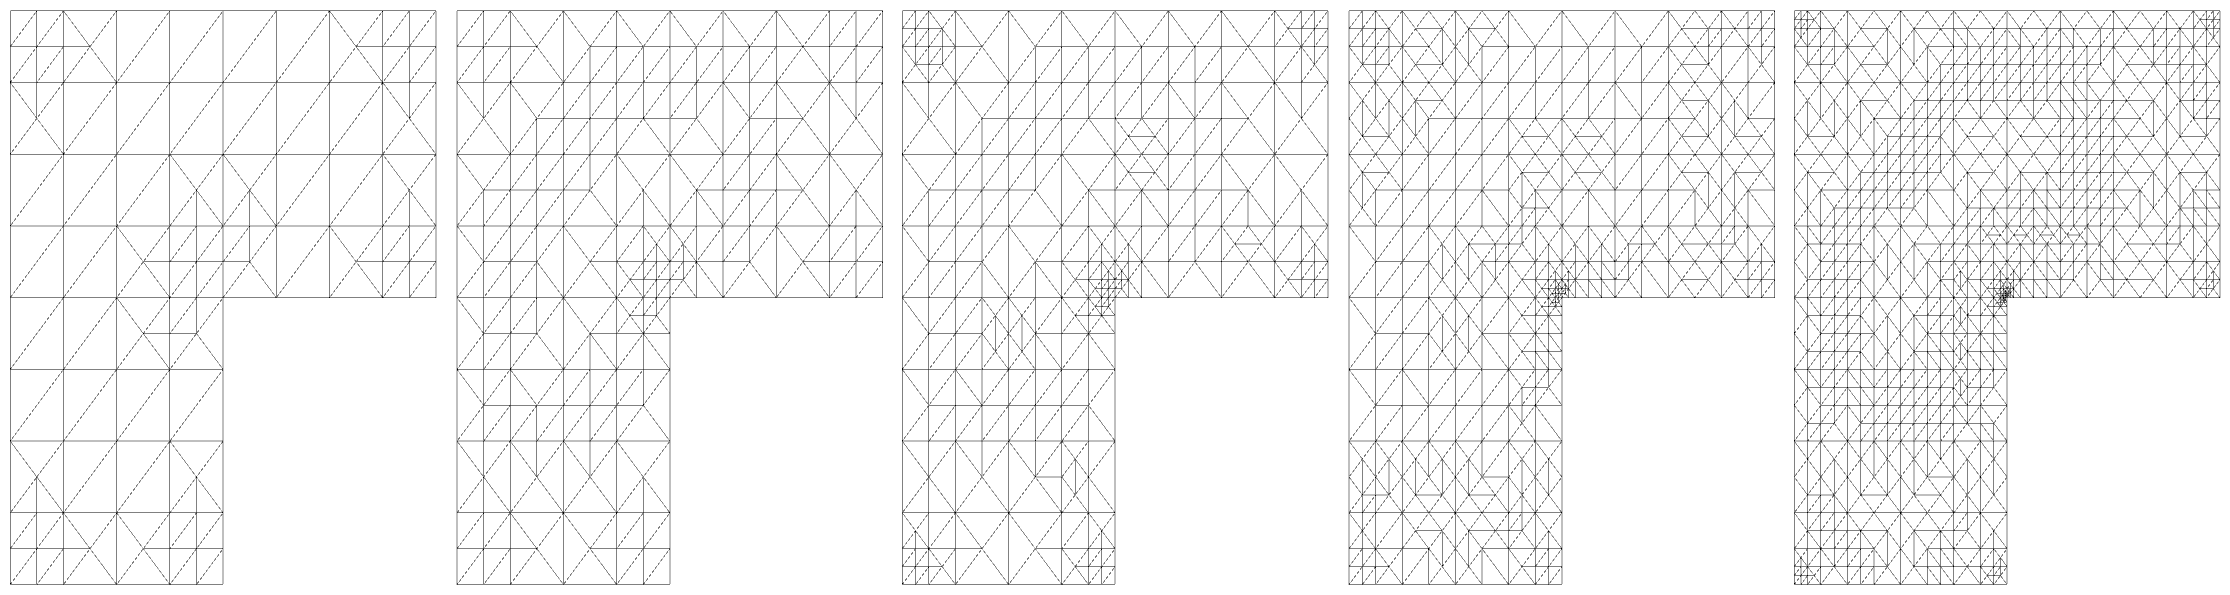
\includegraphics[width=16.5cm,height=3.5cm]{pics/grid05.png} \\
		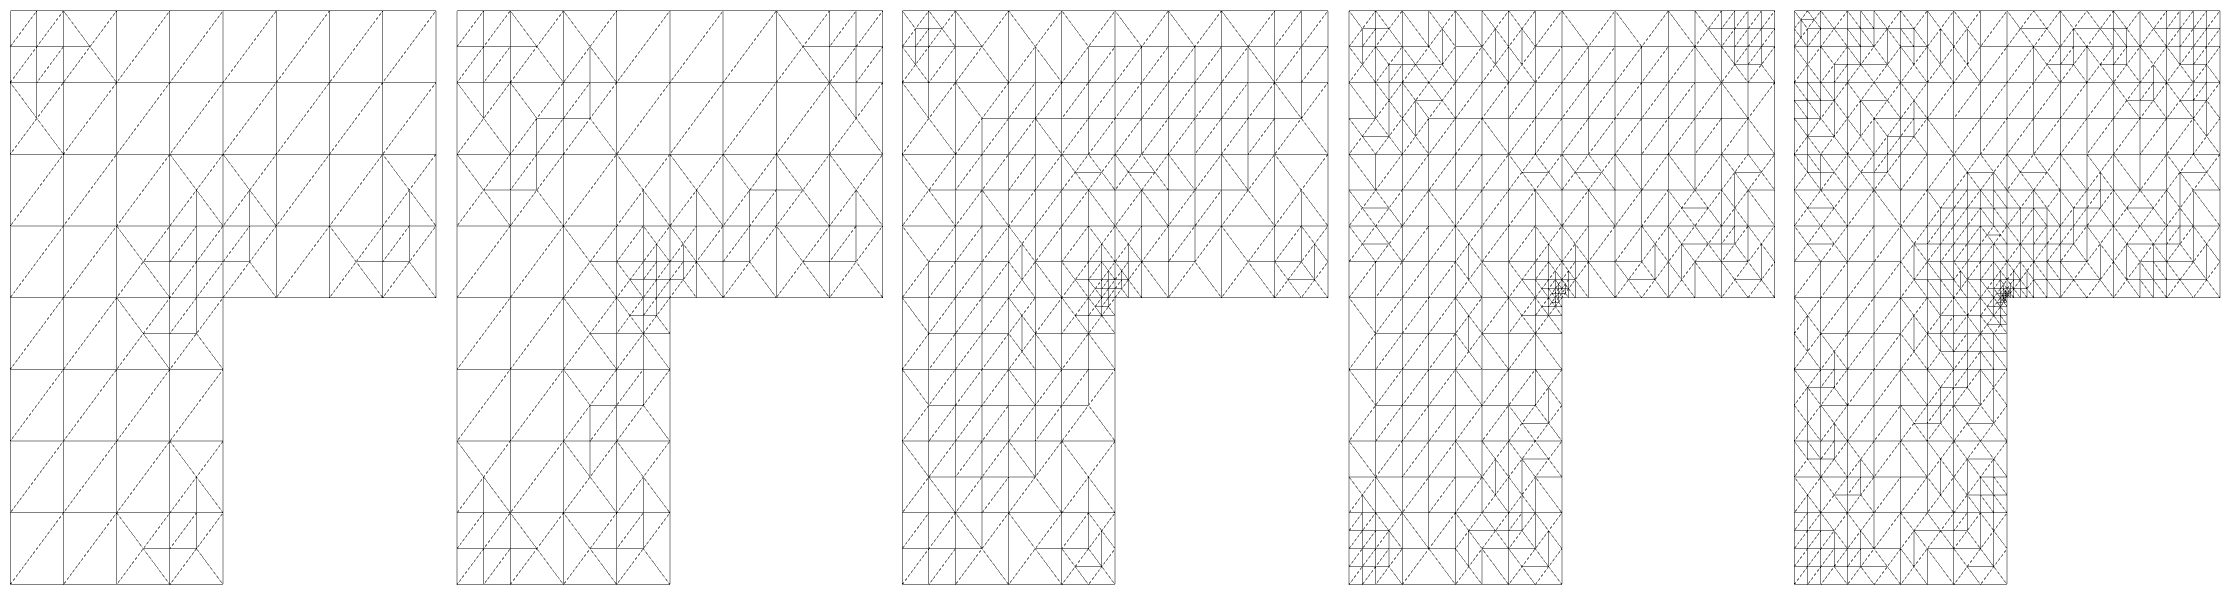
\includegraphics[width=16.5cm,height=3.5cm]{pics/grid06.png} \\
		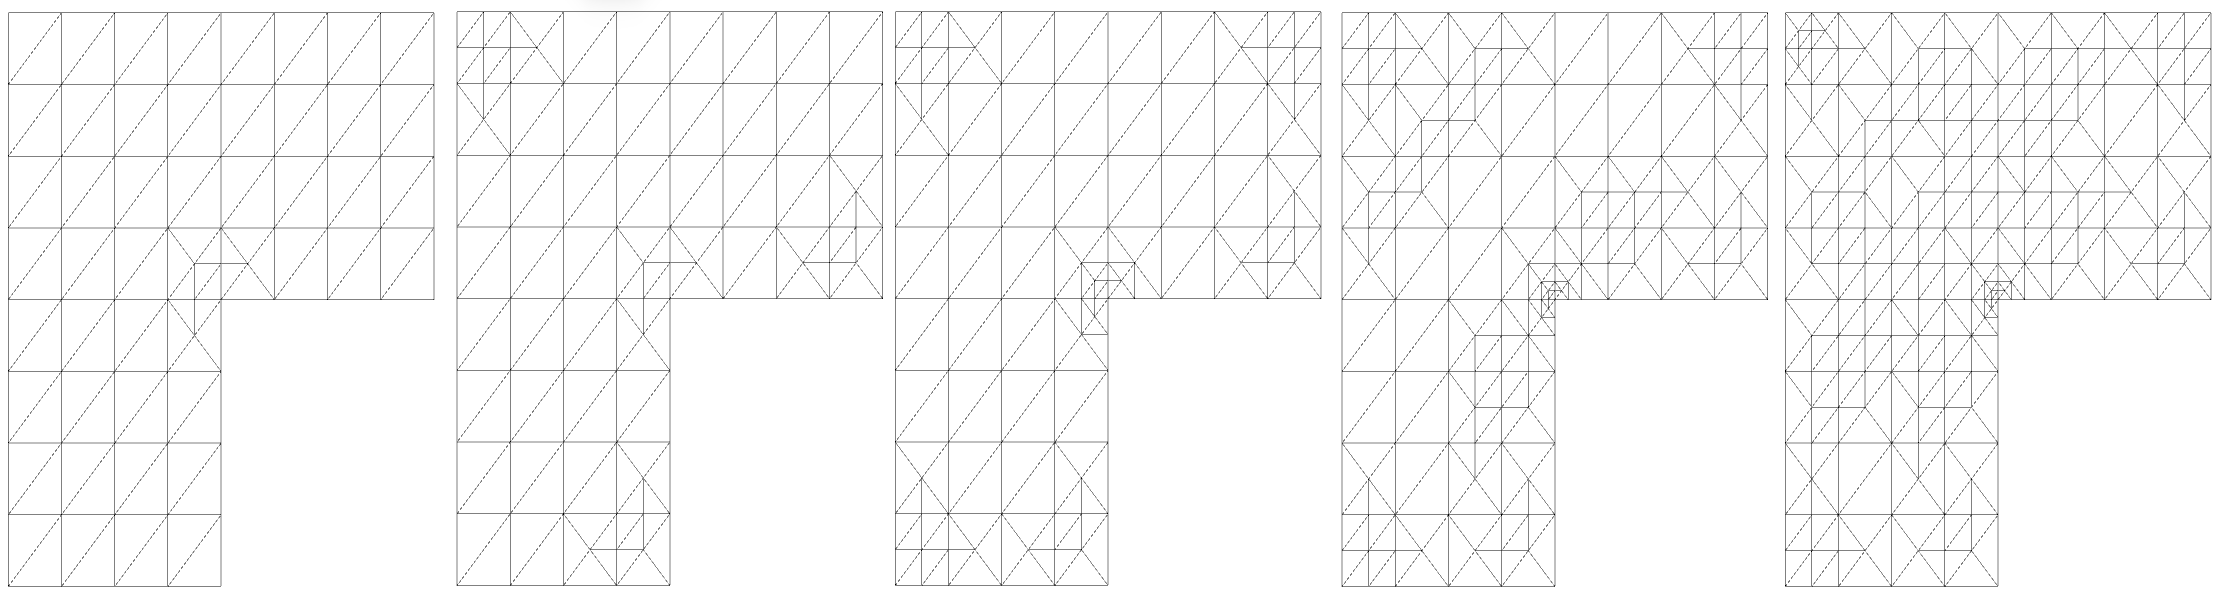
\includegraphics[width=16.5cm,height=3.5cm]{pics/grid08.png} \\
	\end{tabular}
	\caption{ \label{tabelle} Gitterfolgen auf $\Omega_L$ für verschiedene Theta. Von oben nach unten: \newline $\Theta = 0,2/0,4/0,5/0,6/0,8$.}
\end{table}
\begin{figure}[!htbp]
	\begin{center}
		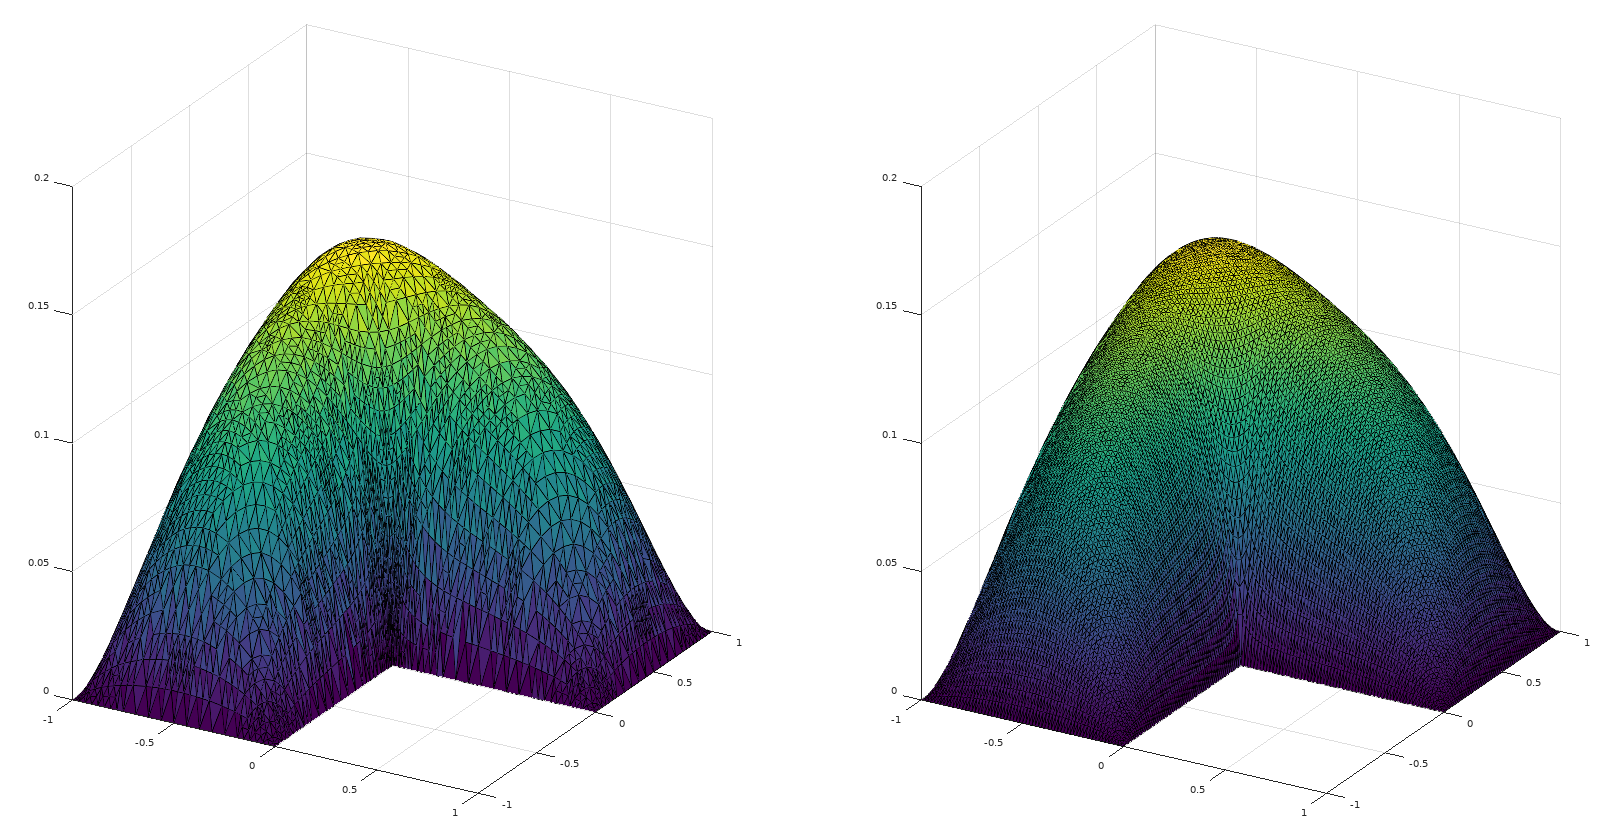
\includegraphics[width=15cm]{pics/approx.PNG}
	\end{center}
	\caption{\label{app} Approximation auf einem adaptiven Gitter auf $\Omega_L$ mit $\Theta = 0,8$ (links) und auf einer Triangulierung mit gleichmäßiger Gitterweite (rechts) mit vergleichbarem Approximationsfehler.}
\end{figure}
\begin{figure}[!htbp]
	\begin{center}
		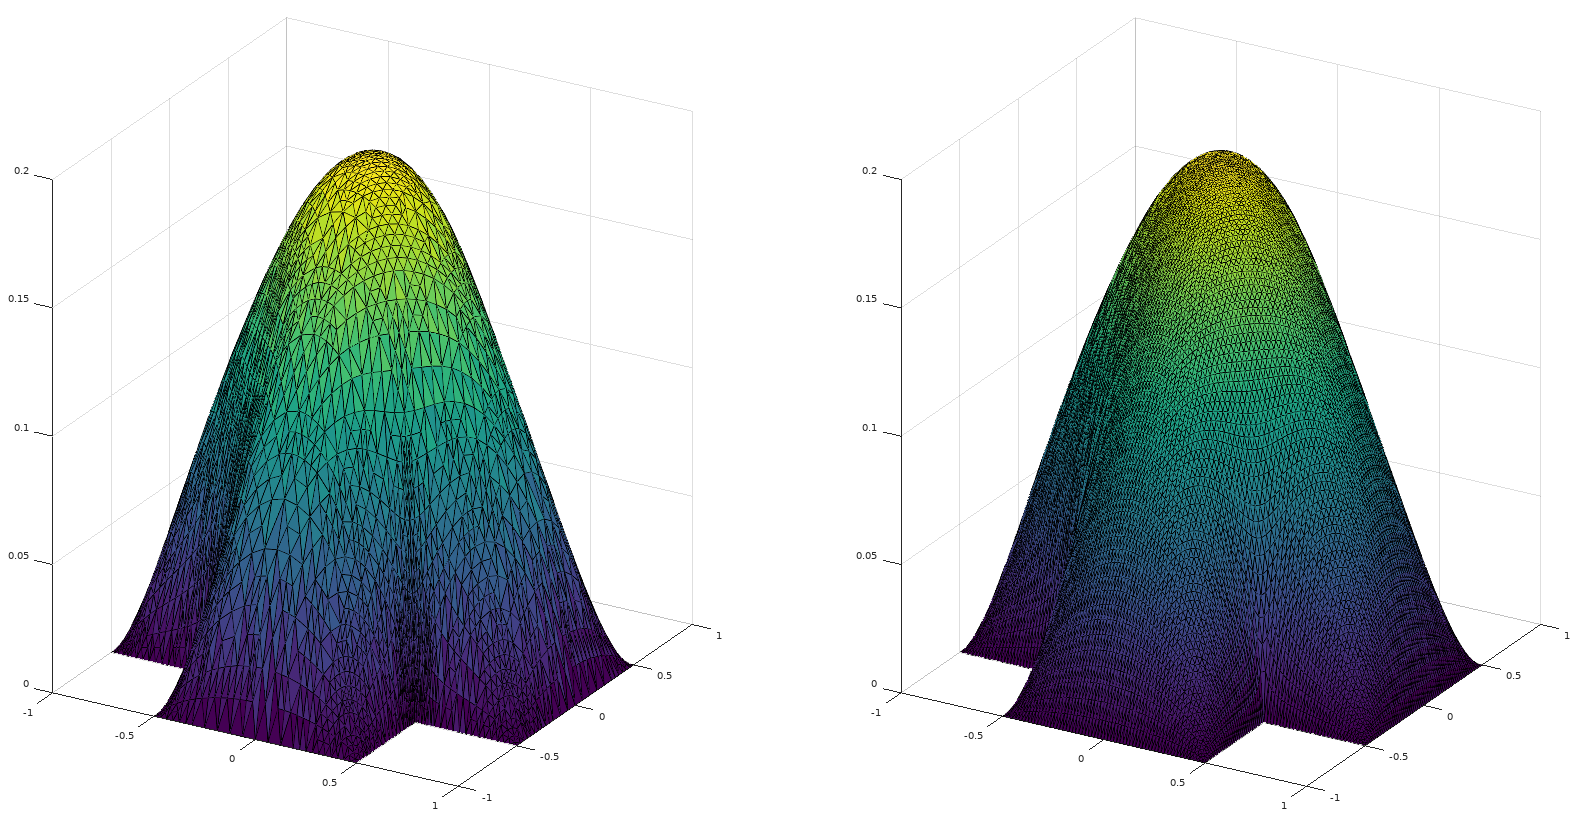
\includegraphics[width=15cm]{pics/approx2.PNG}
	\end{center}
	\caption{\label{app2} Approximation auf einem adaptiven Gitter auf $\Omega_\times$ mit $\Theta = 0,8$ (links) und auf einer Triangulierung mit gleichmäßiger Gitterweite (rechts) mit vergleichbarem Approximationsfehler.}
\end{figure}
